% !TEX encoding = UTF-8
% !TEX TS-program = pdflatex
% !TEX root = ../tesi.tex
% !TEX spellcheck = it-IT

%**************************************************************
\chapter{Analisi dei requisiti}
\label{cap:analisi-requisiti}
%**************************************************************

\intro{}\\

\section{Casi d'uso - lato client}

Per lo studio dei casi di utilizzo del prodotto sono stati creati dei diagrammi.
I diagrammi dei casi d'uso (in inglese \emph{Use Case Diagram}) sono diagrammi di tipo \gls{uml} dedicati alla descrizione delle funzioni o servizi offerti da un sistema, così come sono percepiti e utilizzati dagli attori che interagiscono col sistema stesso.

\begin{figure}[!h] 
    \centering 
    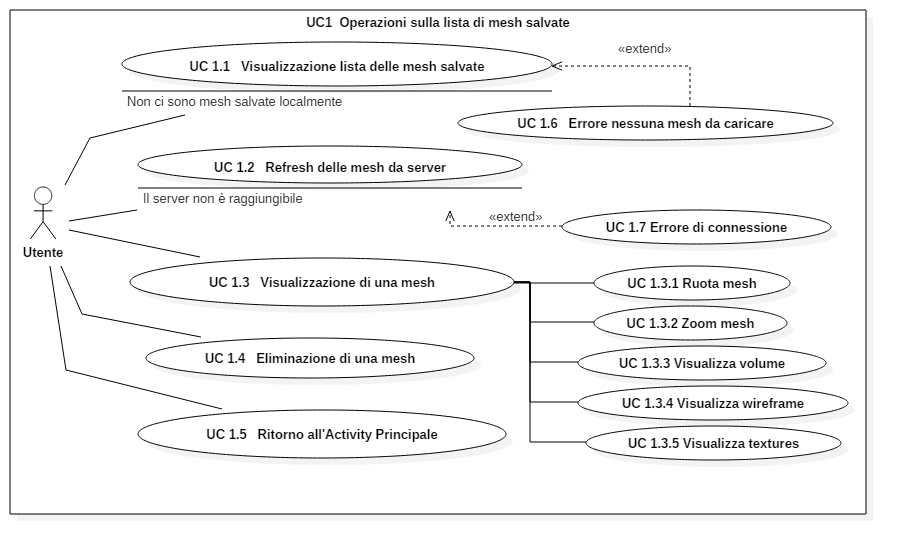
\includegraphics[width=1.0\columnwidth]{usecase/mesh_list} 
    \caption{Use Case - UC1: Operazioni sulla lista di mesh salvate}
\end{figure}

\begin{usecase}{1}{Operazioni sulla lista di mesh salvate}
\usecaseactors{User}
\\ \usecasepre{L'utente ha aperto l'applicazione ed ha premuto sul pulsante per
visualizzare la lista delle mesh 3D salvate localmente}
\\ \usecasedesc{L'utente vede sullo schermo la lista delle mesh 3D salvate su
disco su cui può effettuare diverse azioni}
\\ \usecasepost{Il sistema è pronto per permettere una nuova interazione}
\label{uc:lista-mesh}
\end{usecase}

\subsection{UC1.1: Visualizzazione lista delle mesh salvate}
\textbf{Attori Principali}: Utente.
\\\\ \textbf{Precondizioni}: L'utente ha aperto l'applicazione ed ha premuto sul pulsante per visualizzare la lista delle \emph{mesh} salvate localmente.
\\\\ \textbf{Descrizione}:  L'utente consulta la lista delle \emph{mesh} salvate localmente.
\\\\ \textbf{Postcondizioni}: Viene visualizzata la lista delle mesh salvate localmente.
\\\\ \textbf{Extension Points}:
\begin{itemize}
\item \textbf{Non ci sono mesh salvate localmente}: Non c'è nessuna mesh salvata da caricare in lista, viene visualizzato un messaggio informativo (UC 1.6).
\end{itemize}

\subsection{UC1.2: Refresh delle mesh da server}
\textbf{Attori Principali}: Utente.
\\\\ \textbf{Precondizioni}: L'utente ha aperto l'applicazione, ha premuto sul pulsante per visualizzare la lista delle \emph{mesh} salvate su disco ed ha intenzione di aggiornare la lista di \emph{mesh} aggiungendo le altre presenti sul \emph{Server}.
\\\\ \textbf{Descrizione}: L'utente preme sul simbolo di \emph{refresh} in alto a destra e ricarica la lista di \emph{mesh} eventualmente scaricando quelle sul \emph{Server} ma non sul dispositivo. L'utente viene informato dell'avvenuto refreshing.
\\\\ \textbf{Postcondizioni}: L'utente ha a disposizione una lista aggiornata di \emph{mesh}.
\\\\ \textbf{Extension Points}:
\begin{itemize}
\item \textbf{Il server non è raggiungibile}: c'è stato un errore nel tentativo di connettersi al server. Viene visualizzato un messaggio d'errore (UC 1.7).
\end{itemize}

\subsection{UC1.3: Visualizzazione di una mesh}
\textbf{Attori Principali}: Utente.
\\\\ \textbf{Precondizioni}: L'utente ha aperto l'applicazione, ha premuto sul pulsante per visualizzare la lista delle \emph{mesh} salvate su disco ed intende visualizzare una specifica \emph{mesh} in 3D.
\\\\ \textbf{Descrizione}: L'utente preme sul nome della \emph{mesh} che intende visualizzare, a questo punto si apre un piccolo ambiente grafico 3D dove l'utente può osservare la ricostruzione ed effettuare operazioni su di essa.
\\\\ \textbf{Postcondizioni}: Nessuna.

\subsubsection{UC1.3.1: Ruota mesh}
\textbf{Attori Principali}: Utente.
\\\\ \textbf{Precondizioni}: L'utente sta visualizzando una mesh e vuole ruotarla.
\\\\ \textbf{Descrizione}: L'utente, scorrendo lo schermo con un dito, ruota l'oggetto visualizzato.
\\\\ \textbf{Postcondizioni}: La mesh è stata ruotata.

\subsubsection{UC1.3.2: Zoom mesh}
\textbf{Attori Principali}: Utente.
\\\\ \textbf{Precondizioni}: L'utente sta visualizzando una mesh e vuole ingrandirla/rimpicciolirla.
\\\\ \textbf{Descrizione}: L'utente, usando due dita, ingrandisce/rimpicciolisce l'oggetto visualizzato.
\\\\ \textbf{Postcondizioni}: La mesh è stata ingrandita/rimpicciolita.

\subsubsection{UC1.3.3: Visualizza volume}
\textbf{Attori Principali}: Utente.
\\\\ \textbf{Precondizioni}: L'utente sta visualizzando una mesh e vuole conscerne il volume calcolato.
\\\\ \textbf{Descrizione}: L'utente, cliccando un apposito bottone in alto a destra, visualizza un popup con il volume calcolato della mesh.
\\\\ \textbf{Postcondizioni}: L'utente ha visualizzato il volume della mesh.

\subsubsection{UC1.3.4: Visualizza wireframe}
\textbf{Attori Principali}: Utente.
\\\\ \textbf{Precondizioni}: L'utente sta visualizzando una mesh e vuole osservarne solamente il \emph{wireframe}, cioè lo scheletro di triangoli di cui è composta.
\\\\ \textbf{Descrizione}: L'utente, cliccando un apposito bottone in alto a destra, visualizza solamente il \emph{wireframe} dell'oggetto.
\\\\ \textbf{Postcondizioni}: Viene visualizzato il \emph{wireframe} dell'oggetto.

\subsubsection{UC1.3.5: Visualizza textures}
\textbf{Attori Principali}: Utente.
\\\\ \textbf{Precondizioni}: L'utente sta visualizzando una mesh e vuole applicarvi delle textures di default.
\\\\ \textbf{Descrizione}: L'utente, cliccando un apposito bottone in alto a destra, visualizza la mesh alla quale vengono applicate delle semplici textures di default.
\\\\ \textbf{Postcondizioni}: Viene visualizzata la mesh dell'oggetto, alla quale sono state applicate textures di default.

\subsubsection{UC1.3.6: Ritorno alla lista di mesh}
\textbf{Attori Principali}: Utente.
\\\\ \textbf{Precondizioni}: L'utente sta visualizzando una mesh e desidera ritornare alla lista di mesh.
\\\\ \textbf{Descrizione}: L'utente preme sul tasto "Back" e ritorna alla lista di mesh.
\\\\ \textbf{Postcondizioni}: L'utente è uscito dalla visualizzazione di una mesh ed è ritornato alla lista delle mesh.

\subsection{UC1.4: Eliminazione di una mesh}
\textbf{Attori Principali}: Utente.
\\\\ \textbf{Precondizioni}: L'utente ha aperto l'applicazione, ha premuto sul pulsante per visualizzare la lista delle \emph{mesh} salvate localmente.
\\\\ \textbf{Descrizione}: L'utente preme sul pulsante "Delete" affianco al nome di una specifica mesh per cancellarla dai \emph{File} salvati localmente.
\\\\ \textbf{Postcondizioni}: Il \emph{File} selezionato è stato cancellato e non è più presente sulla memoria del dispositivo.

\subsection{UC1.5: Ritorno all'activity principale}
\textbf{Attori Principali}: Utente.
\\\\ \textbf{Precondizioni}: L'utente ha aperto l'applicazione, ha premuto sul pulsante per visualizzare la lista delle \emph{mesh} salvate su disco ma desidera ritornare all'\emph{activity} principale.
\\\\ \textbf{Descrizione}: L'utente preme sul tasto "Back" e ritorna all'\emph{activity} principale.
\\\\ \textbf{Postcondizioni}: L'utente ritorna all'\emph{activity} principale.

\subsection{UC1.6: Errore nessuna mesh da caricare}
\textbf{Attori Principali}: Utente.
\\\\ \textbf{Precondizioni}: L'utente ha aperto l'applicazione e ha premuto sul pulsante per visualizzare la lista delle \emph{mesh} salvate su disco.
\\\\ \textbf{Descrizione}: L'utente viene informato dell'assenza di mesh salvate localmente.
\\\\ \textbf{Postcondizioni}: La lista di mesh non è stata popolata.

\subsection{UC1.7: Errore di connessione}
\textbf{Attori Principali}: Utente.
\\\\ \textbf{Precondizioni}: L'utente ha selezionato il pulsante di refresh per aggiornare la lista di \emph{mesh} aggiungendo le altre presenti sul \emph{Server}.
\\\\ \textbf{Descrizione}: L'utente viene informato dell'assenza di connessione con il \emph{Server}.
\\\\ \textbf{Postcondizioni}: La comunicazione tra dispositivo e \emph{Server} non è possibile.



\section{Casi d'uso - lato server}
\begin{figure}[!h] 
    \centering 
    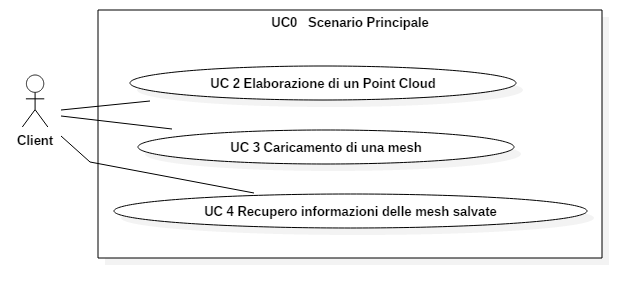
\includegraphics[width=1.0\columnwidth]{usecase/scenario_principale} 
    \caption{Use Case - UC0: Scenario Principale}
\end{figure}

\begin{usecase}{0}{Scenario Principale}
\usecaseactors{Client}
\\ \usecasepre{Il client invia una specifica richiesta al server}
\\ \usecasedesc{Il server elabora la richiesta del client e ne restituisce i risultati}
\\ \usecasepost{Il server ha elaborato la richiesta ed inviato il responso al client}
\label{uc:scenario_principale}
\end{usecase}

\subsection{UC2 Elaborazione di un Point Cloud}
\begin{figure}[!h] 
    \centering 
    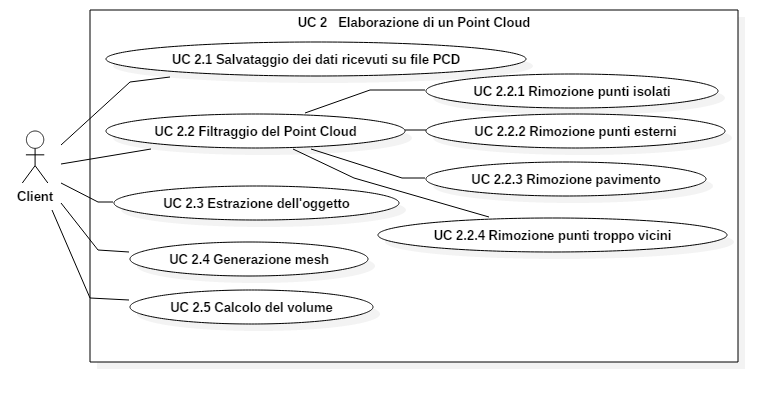
\includegraphics[width=1.0\columnwidth]{usecase/elaborazione} 
    \caption{Use Case - UC2: Elaborazione di un Point Cloud}
\end{figure}

\begin{usecase}{2}{Elaborazione di un Point Cloud}
\usecaseactors{Client}
\\ \usecasepre{Il client richiede l'elaborazione di un Point Cloud al server}
\\ \usecasedesc{Il server elabora il Point Cloud ricevuto e notifica l'esito al client}
\\ \usecasepost{Il client riceve l'esito dell'elaborazione dal server}
\label{uc:elaborazione}
\end{usecase}

\subsection{UC2.1 Salvataggio dei dati ricevuti su file PCD}
\textbf{Attori Principali}: Client.
\\\\ \textbf{Precondizioni}: Il Client invia tramite protocollo HTTP dati in formato PCD.
\\\\ \textbf{Descrizione}: I dati ricevuti vengono salvati sul server in un file in formato PCD.
\\\\ \textbf{Postcondizioni}: I dati sono stati correttamente salvati su file.

\subsection{UC2.2 Filtraggio del Point Cloud}
\textbf{Attori Principali}: Client.
\\\\ \textbf{Precondizioni}: Il Client ha richiesto l'elaborazione di un Point Cloud.
\\\\ \textbf{Descrizione}: Il Point Cloud viene caricato da file e filtrato.
\\\\ \textbf{Postcondizioni}: Il Point Cloud è stato filtrato.

\subsubsection{UC2.2.1 Rimozione punti isolati}
\textbf{Attori Principali}: Client.
\\\\ \textbf{Precondizioni}: Viene richiesto di eliminare i punti isolati della nuvola.
\\\\ \textbf{Descrizione}: Il Point Cloud viene filtrato eliminando i punti isolati.
\\\\ \textbf{Postcondizioni}: I punti isolati sono stati rimossi dal Point Cloud.

\subsubsection{UC2.2.2 Rimozione punti esterni}
\textbf{Attori Principali}: Client.
\\\\ \textbf{Precondizioni}: Viene richiesto di eliminare i punti esterni della nuvola.
\\\\ \textbf{Descrizione}: Il Point Cloud viene filtrato eliminando i punti più esterni, che non appartengono all'oggetto scansionato.
\\\\ \textbf{Postcondizioni}: I punti esterni sono stati rimossi dal Point Cloud.

\subsubsection{UC2.2.3 Rimozione pavimento}
\textbf{Attori Principali}: Client.
\\\\ \textbf{Precondizioni}: Viene richiesto di eliminare i punti del pavimento dalla nuvola.
\\\\ \textbf{Descrizione}: Il Point Cloud viene filtrato eliminando i punti planari che corrispondono al pavimento.
\\\\ \textbf{Postcondizioni}: I punti del pavimento sono stati rimossi dal Point Cloud.

\subsubsection{UC2.2.4 Rimozione punti troppo vicini}
\textbf{Attori Principali}: Client.
\\\\ \textbf{Precondizioni}: Viene richiesto di eliminare i punti ravvicinati della nuvola.
\\\\ \textbf{Descrizione}: Il Point Cloud viene filtrato eliminando i punti eccessivamente ravvicinati, che possono essere approssimati in un unico punto.
\\\\ \textbf{Postcondizioni}: I punti ravvicinati sono stati rimossi dal Point Cloud.

\subsection{UC2.3 Estrazione dell'oggetto}
\textbf{Attori Principali}: Client.
\\\\ \textbf{Precondizioni}: Viene richiesto di estrarre dalla nuvola i soli punti appartenenti all'oggetto scansionato.
\\\\ \textbf{Descrizione}: La parte di Point Cloud che rappresenta l'oggetto scansionato viene isolata dal resto dei punti.
\\\\ \textbf{Postcondizioni}: I punti del solo oggetto scansionato sono stati estratti dal Point Cloud.

\subsection{UC2.4 Generazione mesh}
\textbf{Attori Principali}: Client.
\\\\ \textbf{Precondizioni}: Il Client richiede di generare una mesh dell'oggetto ispezionato.
\\\\ \textbf{Descrizione}: Viene effettuato il meshing del Point Cloud del solo oggetto scansionato.
\\\\ \textbf{Postcondizioni}: \'E stata generata correttamente una mesh dell'oggetto ispezionato.

\subsection{UC2.5 Calcolo del volume}
\textbf{Attori Principali}: Client.
\\\\ \textbf{Precondizioni}: il Client richiede di calcolare il volume dell'oggetto scansionato.
\\\\ \textbf{Descrizione}: Viene calcolato il volume della mesh generata a partire dal Point Cloud.
\\\\ \textbf{Postcondizioni}: Il volume dell'oggetto è stato calcolato.

%%%%%%%%%%%%%%%%%%%%%%%%%%%%%%%%%%%%%%%%%%%%%%%%%%%%%%%%%%%%%%%%%%%

\subsection{UC3 Caricamento di una mesh}
\begin{figure}[!h] 
    \centering 
    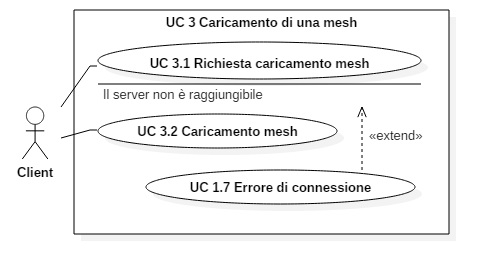
\includegraphics[width=0.9\columnwidth]{usecase/caricamento} 
    \caption{Use Case - UC3: Caricamento di una mesh}
\end{figure}

\begin{usecase}{3}{Caricamento di una mesh}
\usecaseactors{Client}
\\ \usecasepre{Il client richiede al server l'invio di una specifica mesh}
\\ \usecasedesc{Il server elabora la richiesta ricevuta ed invia la mesh desiderata al Client}
\\ \usecasepost{Il client riceve la mesh richiesta dal server}
\label{uc:caricamento}
\end{usecase}

\subsection{UC3.1 Richiesta caricamento Mesh}
\textbf{Attori Principali}: Client.
\\\\ \textbf{Precondizioni}: Il Client richiede il caricamento di una mesh inviando tramite protocollo HTTP il nome della mesh richiesta.
\\\\ \textbf{Descrizione}: Il server elabora la richiesta e si appresta ad inviare il file richiesto.
\\\\ \textbf{Postcondizioni}: Il server ha ricevuto la richiesta e si appresta ad inviare il file richiesto.
\\\\ \textbf{Extension Points}:
\begin{itemize}
\item \textbf{Il server non è raggiungibile}: c'è stato un errore nel tentativo di connettersi al server. Viene visualizzato un messaggio d'errore (UC 1.7).
\end{itemize}

\subsection{UC3.2 Caricamento Mesh}
\textbf{Attori Principali}: Client.
\\\\ \textbf{Precondizioni}: Il Client ha inviato il nome della mesh da caricare .
\\\\ \textbf{Descrizione}: Il server legge il file OBJ della mesh e lo invia al Client.
\\\\ \textbf{Postcondizioni}: Il client riceve la mesh richiesta.

%%%%%%%%%%%%%%%%%%%%%%%%%%%%%%%%%%%%%%%%%%%%%%%%%%%%%%%%%%%%%%%%%%%
\newpage
\subsection{UC4 Caricamento informazioni delle mesh salvate}
\begin{figure}[!h] 
    \centering 
    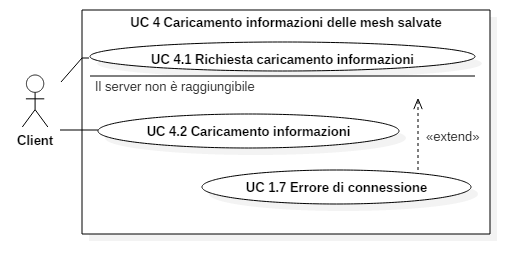
\includegraphics[width=0.9\columnwidth]{usecase/informazioni} 
    \caption{Use Case - UC4: Caricamento informazioni delle mesh salvate}
\end{figure}

\begin{usecase}{4}{Caricamento informazioni delle mesh salvate}
\usecaseactors{Client}
\\ \usecasepre{Il client richiede una lista di informazioni quali nome, data di creazione e volume delle mesh salvate su server}
\\ \usecasedesc{Il server elabora la richiesta ricevuta ed invia le informazioni al client}
\\ \usecasepost{Il client riceve le informazioni richieste dal server}
\label{uc:informazioni}
\end{usecase}

\subsection{UC4.1 Richiesta caricamento informazioni}
\textbf{Attori Principali}: Client.
\\\\ \textbf{Precondizioni}: Il Client richiede informazioni sulle mesh salvate nel server inviando una richiesta tramite protocollo HTTP.
\\\\ \textbf{Descrizione}: Il server elabora la richiesta e si appresta ad inviare le informazioni richieste.
\\\\ \textbf{Postcondizioni}: Il server ha ricevuto la richiesta e si appresta a recuperare ed inviare le informazioni.
\\\\ \textbf{Extension Points}:
\begin{itemize}
\item \textbf{Il server non è raggiungibile}: c'è stato un errore nel tentativo di connettersi al server. Viene visualizzato un messaggio d'errore (UC 1.7).
\end{itemize}

\subsection{UC4.2 Caricamento informazioni}
\textbf{Attori Principali}: Client.
\\\\ \textbf{Precondizioni}: Il Client ha richiesto l'invio di informazioni sulle mesh salvate nel server.
\\\\ \textbf{Descrizione}: Il server recupera le informazioni richieste dalle mesh disponibili e le invia al Client.
\\\\ \textbf{Postcondizioni}: Il client riceve le informazioni richieste.


\section{Requisiti}

Da un'attenta analisi dei requisiti e degli use case effettuata sul progetto è stata stilata la tabella che traccia i requisiti in rapporto agli use case.\\
Sono stati individuati diversi tipi di requisiti e si è quindi fatto utilizzo di un codice identificativo per distinguerli.\\
Il codice dei requisiti è così strutturato R(F/Q/V)(N/D/O) dove:
\begin{enumerate}
	\item[R =] requisito
    \item[F =] funzionale
    \item[Q =] qualitativo
    \item[V =] di vincolo
    \item[O =] obbligatorio
    \item[D =] desiderabile
    \item[Z =] opzionale
\end{enumerate}
Nelle tabelle \ref{tab:requisiti-funzionali}, \ref{tab:requisiti-qualitativi} e \ref{tab:requisiti-vincolo} sono riassunti i requisiti e il loro tracciamento con gli use case delineati in fase di analisi.

\subsection{Requisiti Funzionali}
\LTXtable{\textwidth}{tabelle/funzionali.tex}

\subsection{Requisiti Qualitativi}
\LTXtable{\textwidth}{tabelle/qualitativi.tex}

\subsection{Requisiti di Vincolo}
\LTXtable{\textwidth}{tabelle/vincolo.tex}

\subsection{Requisiti Prestazionali}
\LTXtable{\textwidth}{tabelle/prestazionali.tex}